\documentclass[11pt]{article}

\usepackage{graphicx}
\usepackage{color}
\usepackage{algorithm}
\usepackage{algpseudocode}

\usepackage[T1]{fontenc}
\usepackage[utf8]{inputenc}
\usepackage{indentfirst}

\usepackage[justification=centering]{caption}

\usepackage{amsmath}
\usepackage{amssymb}
\usepackage{dsfont}

\usepackage{multicol}
\usepackage{url}
\usepackage[hmarginratio=1:1,top=15mm,left=15mm,right=15mm,bottom=15mm,columnsep=15pt]{geometry}
\usepackage{siunitx}

\setlength{\parskip}{1em}

\title{HW3 $-$ Stationary solutions of the 1D Schrödinger equation}
\author{Enrique Gómez Cruz\\Facultad de Ciencias, Universidad Nacional Autónoma de México.}
\date{}

\begin{document}
\maketitle
  
The quantum harmonic oscillator is
\begin{equation*}
  \left(-\frac{\hbar}{2m} \frac{d^2}{dz^2}+\frac{1}{2}m\omega z^2 \right)\psi(z) = E\psi(z)
\end{equation*}
This equation is perfectly suited to be solved with the Numerov algorithm since it is of the form
\begin{equation*}
  f'' + k(x) f = 0
\end{equation*}

By introducing a change of variable and scaling the energy with the following definitions
\begin{equation*}
  E\equiv \epsilon\hbar\omega \qquad z\equiv \sqrt{\frac{\hbar}{m\omega}} x
\end{equation*}

We get a dimensionless form of the quantum harmonic oscillator
\begin{equation}
  \psi''+(2\epsilon - x^2)\psi = 0
  \label{eqn:qho}
\end{equation}
Where the dimensionless energy is $\epsilon$ and the scaled potential is $v(x) = x^2/2$

To see if a given energy was an eigenenergy we applied Numerov to equation~\ref{eqn:qho} to get a discrete form of the wave function $\psi$.  If we have an eigenenergy then the tail of the wavefunction must oblige to the border conditions $\psi(x_0) = 0$ and $\psi(x_N) = 0$, where $x_0$ and $x_N$ define the borders where the wave function must vanish.

By construction, our implementation of the Numerov algorithm assures that the border condition $\psi(x_0) = 0$ is always true. But the other border condition must be checked by testing if the tail of the wavefunction doesn't diverge.

The program \textit{schrodingerEquation1D-Numerov.cpp} shows the energies for which the border conditions are true. If you run the program you can see that this are of the form
\begin{equation*}
  \epsilon = n +\frac{1}{2}\text{, } n \in \mathds{N}
\end{equation*}

The next figures show some of the eigenfunctions found.
\begin{figure}[H]
  \centering
  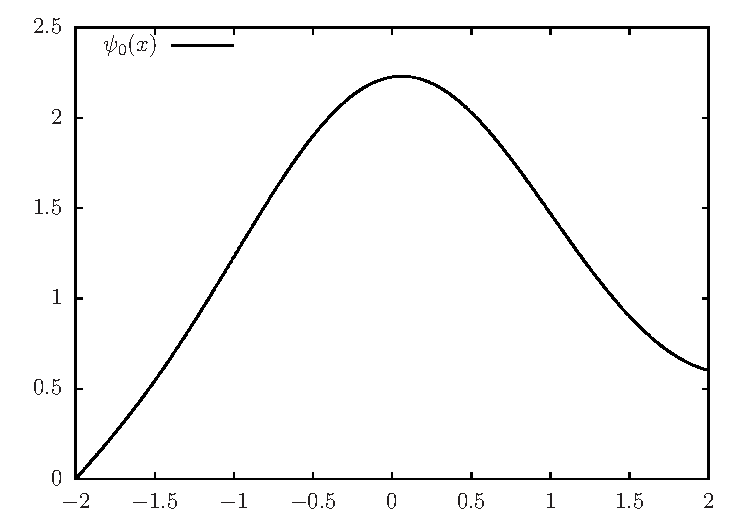
\includegraphics[width=.7\linewidth]{schrodinger-n0}
  \caption{Ground state eigenfunction.}
  \label{fig:schrodinger-n0}
\end{figure}

\begin{figure}[H]
  \centering
  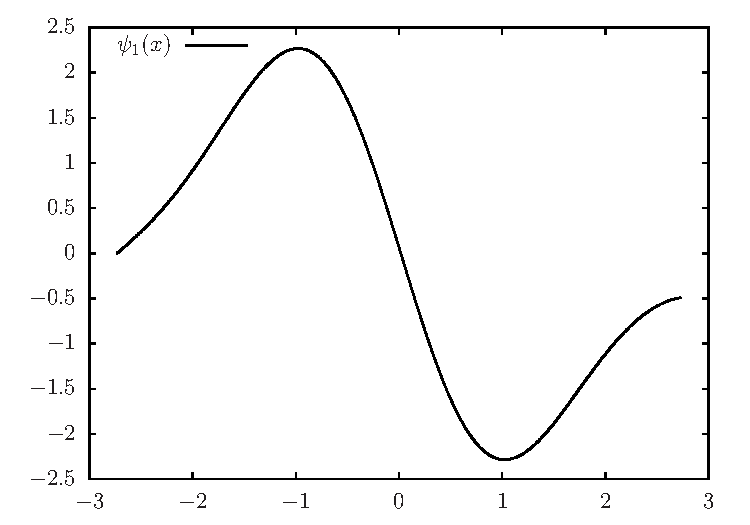
\includegraphics[width=.7\linewidth]{schrodinger-n1}
  \caption{Wave function for $n=1$}
  \label{fig:schrodinger-n1}
\end{figure}

\begin{figure}[H]
  \centering
  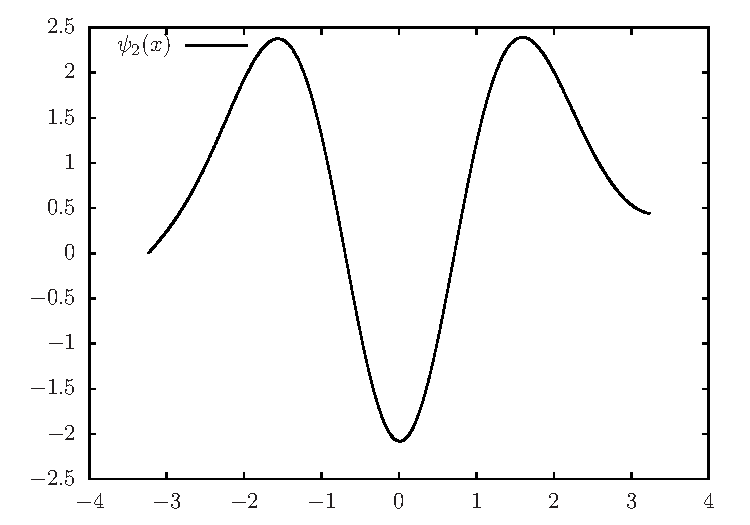
\includegraphics[width=.7\linewidth]{schrodinger-n2}
  \caption{Wave function for $n=2$}
  \label{fig:schrodinger-n2}
\end{figure}
\begin{figure}[H]
  \centering
  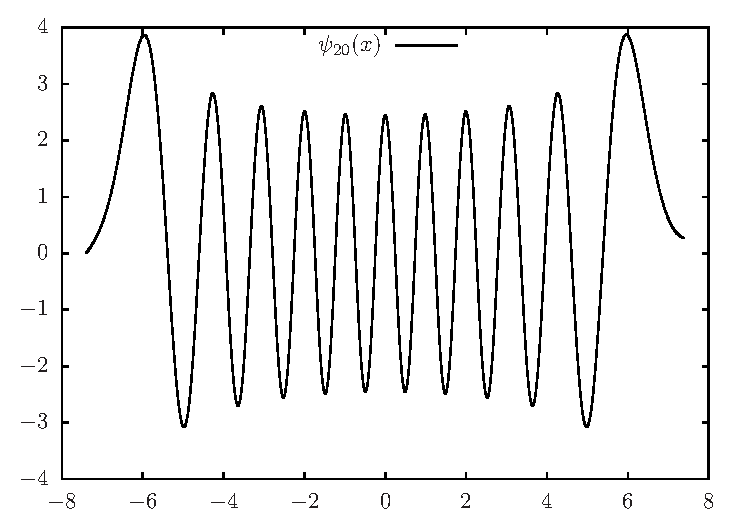
\includegraphics[width=.7\linewidth]{schrodinger-n20}
  \caption{Wave function for $n=20$}
  \label{fig:schrodinger-n20}
\end{figure}
\begin{figure}[H]
  \centering
  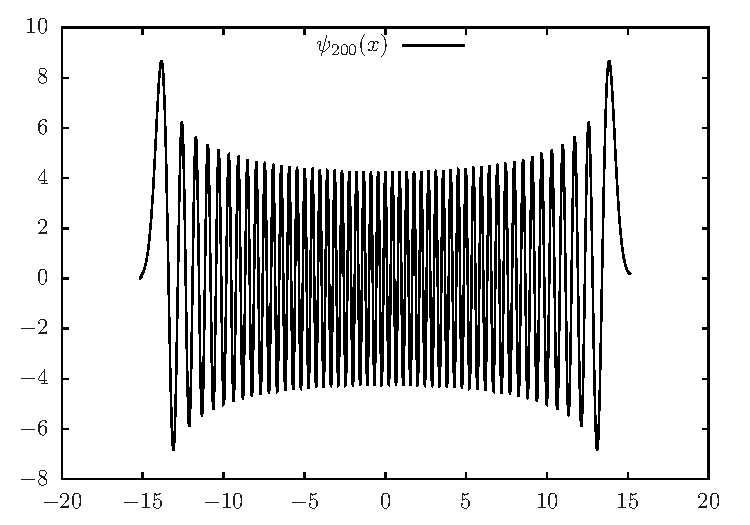
\includegraphics[width=.7\linewidth]{schrodinger-n200}
  \caption{Wave function for $n=200$}
  \label{fig:schrodinger-n200}
\end{figure}

\begin{figure}[H]
  \centering
  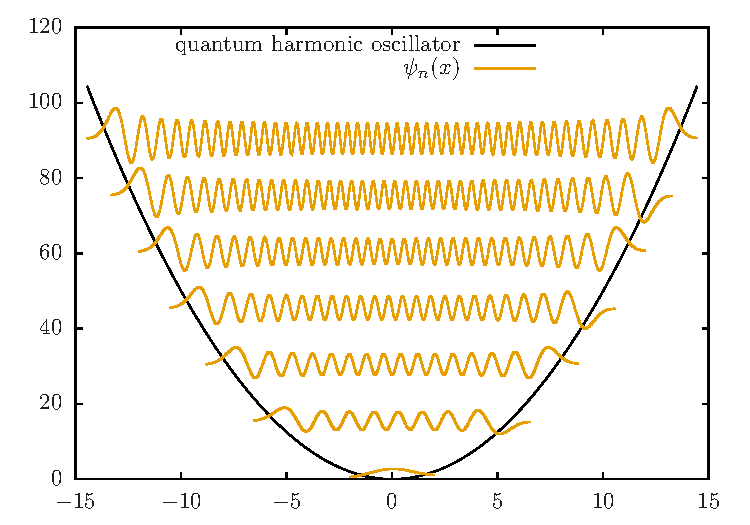
\includegraphics[width=.7\linewidth]{schrodinger-n}
  \caption{Scaled potential for the quantum harmonic oscillator and some eigenfuncions}
  \label{fig:schrodinger-n}
\end{figure}
\end{document}
